% Pulling a 1-form alpha back along a curve c from [a,b] into U.
% Source: book/tex/diffgeo/stokes.tex (§ Pullback of differential forms).
\documentclass[border=2mm]{standalone}
\usepackage{tikz}\usetikzlibrary{arrows.meta}\usepackage{amssymb}
\begin{document}
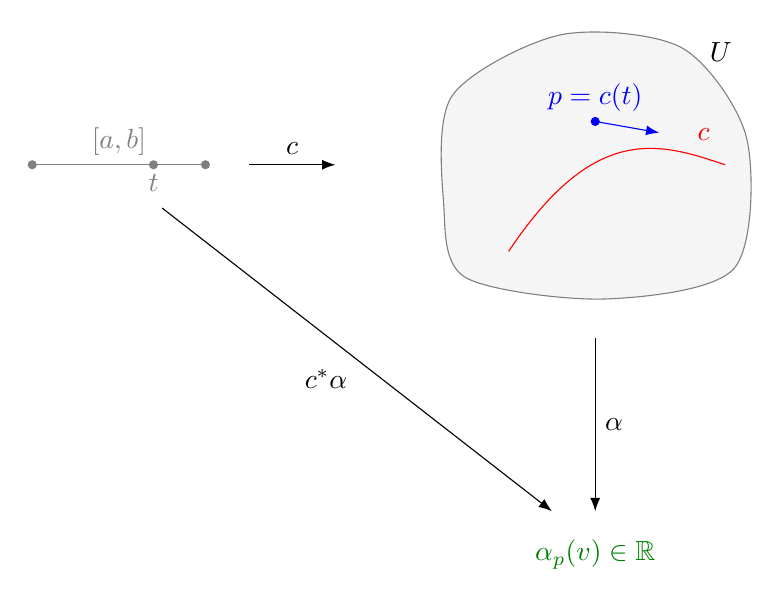
\begin{tikzpicture}[scale=0.55,>={Latex}]
  \draw[gray] (-13,0)--(-9,0); \fill[gray](-13,0)circle(3pt);\fill[gray](-9,0)circle(3pt);
  \node[gray,above] at (-11,0){$[a,b]$}; \fill[gray](-10.2,0)circle(3pt) node[gray,below]{$t$};
  \draw[->] (-8,0)--(-6,0) node[midway,above]{$c$};
  \draw[gray,fill=gray!8] plot[smooth cycle] coordinates {(-3,-2.6)(0.2,-3.1)(3.2,-2.4)(3.5,0.6)(2,2.7)(-0.8,3)(-3.3,1.6)(-3.5,-0.9)};
  \node at (2.9,2.6){$U$};
  \draw[red] (-2,-2) .. controls (0,1) and (1.5,0.5) .. (3,0); \node[red] at (2.5,0.7){$c$};
  \fill[blue] (0,1)circle(3pt) node[blue,above]{$p=c(t)$};
  \draw[blue,->] (0,1)--(1.48,0.74);
  \draw[->] (0,-4)--(0,-8) node[midway,right]{$\alpha$};
  \node[green!50!black] at (0,-9){$\alpha_p(v)\in\mathbb{R}$};
  \draw[->] (-10,-1)--(-1,-8); \node[below left] at (-5.5,-4.5){$c^\ast\alpha$};
\end{tikzpicture}
\end{document}
